\documentclass[mathserif]{beamer}
\usepackage{graphicx}
\usepackage{epstopdf}
\usecolortheme{dove}

\title{Moving Target Indicator}
\author{Chakradhar Thallapaka (09007046) \\ Swrangsar Basumatary (09d07040) }
\institute{Department of Electrical Engineering \\ IIT Bombay, Powai}
\date{April 25, 2014}

    
\begin{document}
    \frame{\titlepage}
    
    
    \begin{frame}{Moving Target Indicator}
      \begin{minipage}[t][0.8\textheight][t]{\textwidth}    	
    	\begin{itemize}
		    \item mode of operation of radar
		    \item makes use of doppler effect
	    \end{itemize}
    	\begin{figure}[h]
    		\centering
    		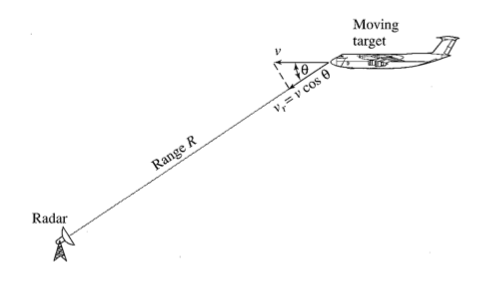
\includegraphics[width=0.7\linewidth]{mti} 
    	\end{figure}
	\vfill
	\tiny{Source: Merrill I.~Skolnik. \emph{Introduction to Radar Systems}. McGraw-Hill, 2001.}
      \end{minipage}
    \end{frame}

    
    \begin{frame}{Single Delay Line Canceler}
      \begin{minipage}[t][0.8\textheight][t]{\textwidth}
	\begin{figure}[h]
		\centering
		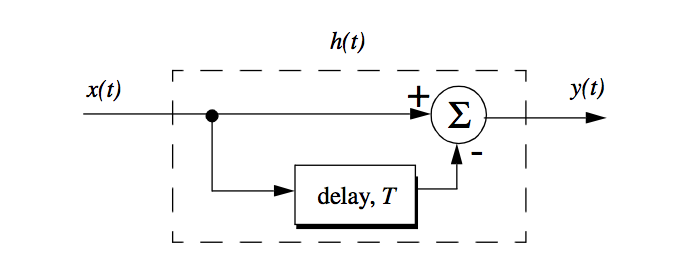
\includegraphics[width=\linewidth]{singleDLC} 
	\end{figure}
	\vfill
	\tiny{Source: Bassem R.~Mahafza. \emph{Radar Systems Analysis and Design Using MATLAB\textsuperscript{\textregistered}}. Chapman \& Hall/CRC, 2000.} 
      \end{minipage}
    \end{frame}
    

    \begin{frame}{Single Delay Line Canceler}
      \begin{minipage}[t][0.8\textheight][t]{\textwidth}
   	\begin{align}
    	 h(t) & = \delta(t) - \delta(t-T) \nonumber \\
    	 H(\omega) & = 1 - e^{-j\omega T} \nonumber \\
    	 |H(\omega)|^2 & = H(\omega)H^*(\omega) \nonumber \\
    	 & = (1 - e^{-j\omega T})(1 - e^{j\omega T}) \nonumber \\
    	 & = 2(1-cos\omega T) \nonumber \\
    	 & = 4(sin(\omega T/2))^2 \nonumber
    	\end{align}
	\vfill
   	\tiny{Source: Bassem R.~Mahafza. \emph{Radar Systems Analysis and Design Using MATLAB\textsuperscript{\textregistered}}. Chapman \& Hall/CRC, 2000.}
      \end{minipage}
    \end{frame}
    
    
    \begin{frame}{Double Delay Line Canceler}
      \begin{minipage}[t][0.8\textheight][t]{\textwidth}
	\begin{figure}[h]
		\centering
		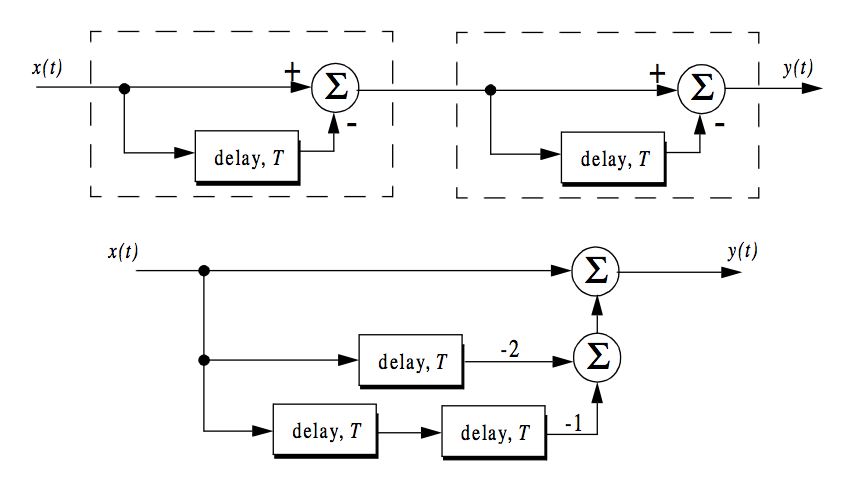
\includegraphics[width=0.8\linewidth]{doubleDLC} 
		\caption{Two configurations for a double delay line canceler}
	\end{figure}
	\vfill
    	\tiny{Source: Bassem R.~Mahafza. \emph{Radar Systems Analysis and Design Using MATLAB\textsuperscript{\textregistered}}. Chapman \& Hall/CRC, 2000.}
      \end{minipage}
    \end{frame}
    
    
    \begin{frame}{Double Delay Line Canceler}
      \begin{minipage}[t][0.8\textheight][t]{\textwidth}
	\begin{align}
	  h(t) & = \delta(t) - 2\delta(t-T) + \delta(t-2T) \nonumber \\
	  |H(\omega)|^2 & = |H_1(\omega)|^2|H_1(\omega)|^2 \nonumber \\
	  & where~ |H_1(\omega)|^2 = 4(sin(\omega T/2))^2 \nonumber \\
	  |H(\omega)|^2 & = 16\left(sin\left(\omega\frac{T}{2}\right)\right)^4 \nonumber
	\end{align}
	\vfill
    	\tiny{Source: Bassem R.~Mahafza. \emph{Radar Systems Analysis and Design Using MATLAB\textsuperscript{\textregistered}}. Chapman \& Hall/CRC, 2000.}
      \end{minipage}
    \end{frame}



    \begin{frame}{Delay Line Canceler}
    	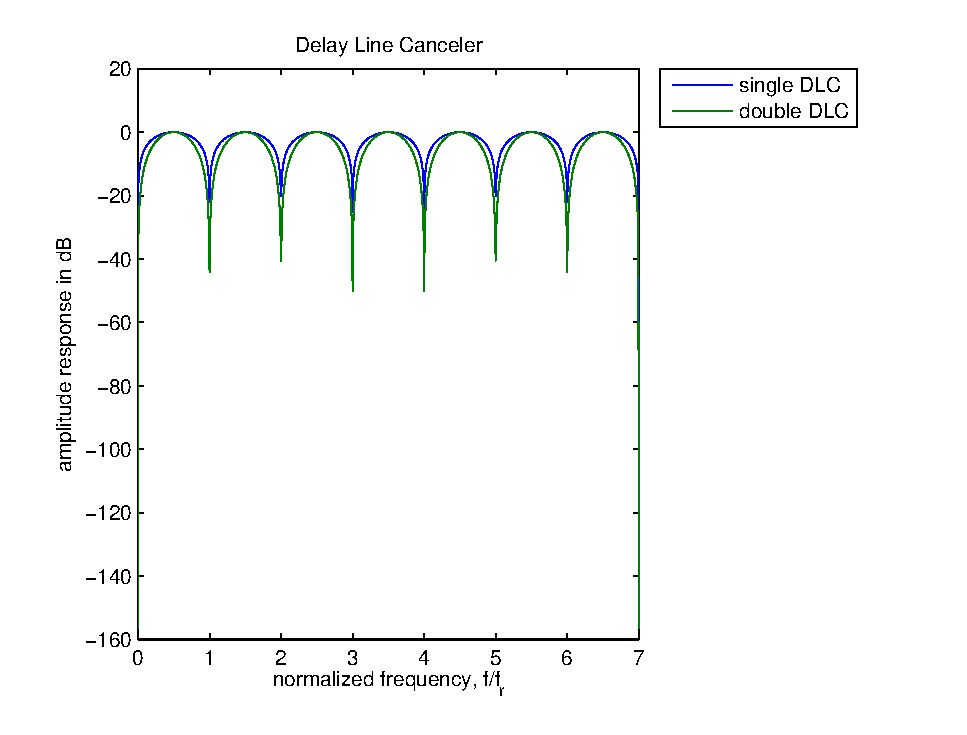
\includegraphics[width=\linewidth]{delayLineCanceler}
    \end{frame}
    
    
    
    \begin{frame}{Delay Lines with Feedback}
      \begin{minipage}[t][0.8\textheight][t]{\textwidth}
	\begin{figure}[h]
		\centering
		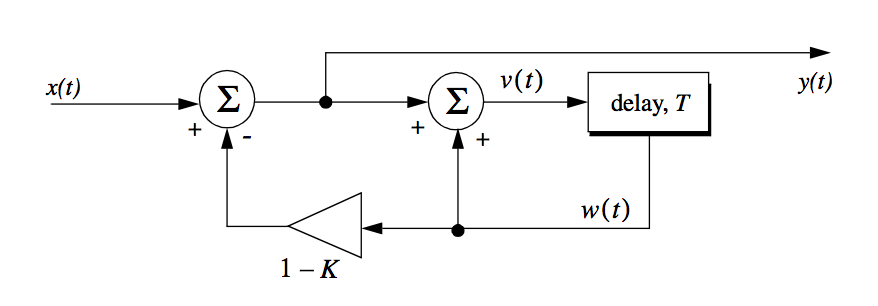
\includegraphics[width=0.8\linewidth]{feedbackDLC} 
		\caption{MTI recursive filter}
	\end{figure}
	\vfill
	\tiny{Here, K is the gain factor.} \\
    	\tiny{Source: Bassem R.~Mahafza. \emph{Radar Systems Analysis and Design Using MATLAB\textsuperscript{\textregistered}}. Chapman \& Hall/CRC, 2000.}
      \end{minipage}
    \end{frame}
    
    
    
    \begin{frame}{Delay Lines with Feedback}
      \begin{minipage}[t][0.8\textheight][t]{\textwidth}
	\begin{align}
	  H(z) & = \frac{1 - z^{-1}}{1-Kz^{-1}} \nonumber \\
	  |H(z)|^2 & = \frac{(1-z^{-1})(1-z)}{(1-Kz^{-1})(1-Kz)} \nonumber \\
	  & = \frac{2-(z+z^{-1})}{(1+K^2)-K(z+z^{-1})} \nonumber \\
	  \left|{H(e^{j\omega T})}\right|^2 & = \frac{2(1-cos\omega T)}{(1+K^2)-2Kcos(\omega T)} \nonumber
	\end{align}
	\vfill
	\tiny{Source: Bassem R.~Mahafza. \emph{Radar Systems Analysis and Design Using MATLAB\textsuperscript{\textregistered}}. Chapman \& Hall/CRC, 2000.}
      \end{minipage}
    \end{frame}
    
    
    \begin{frame}{Delay Lines with Feedback}
      \begin{minipage}[t][0.8\textheight][t]{\textwidth}
	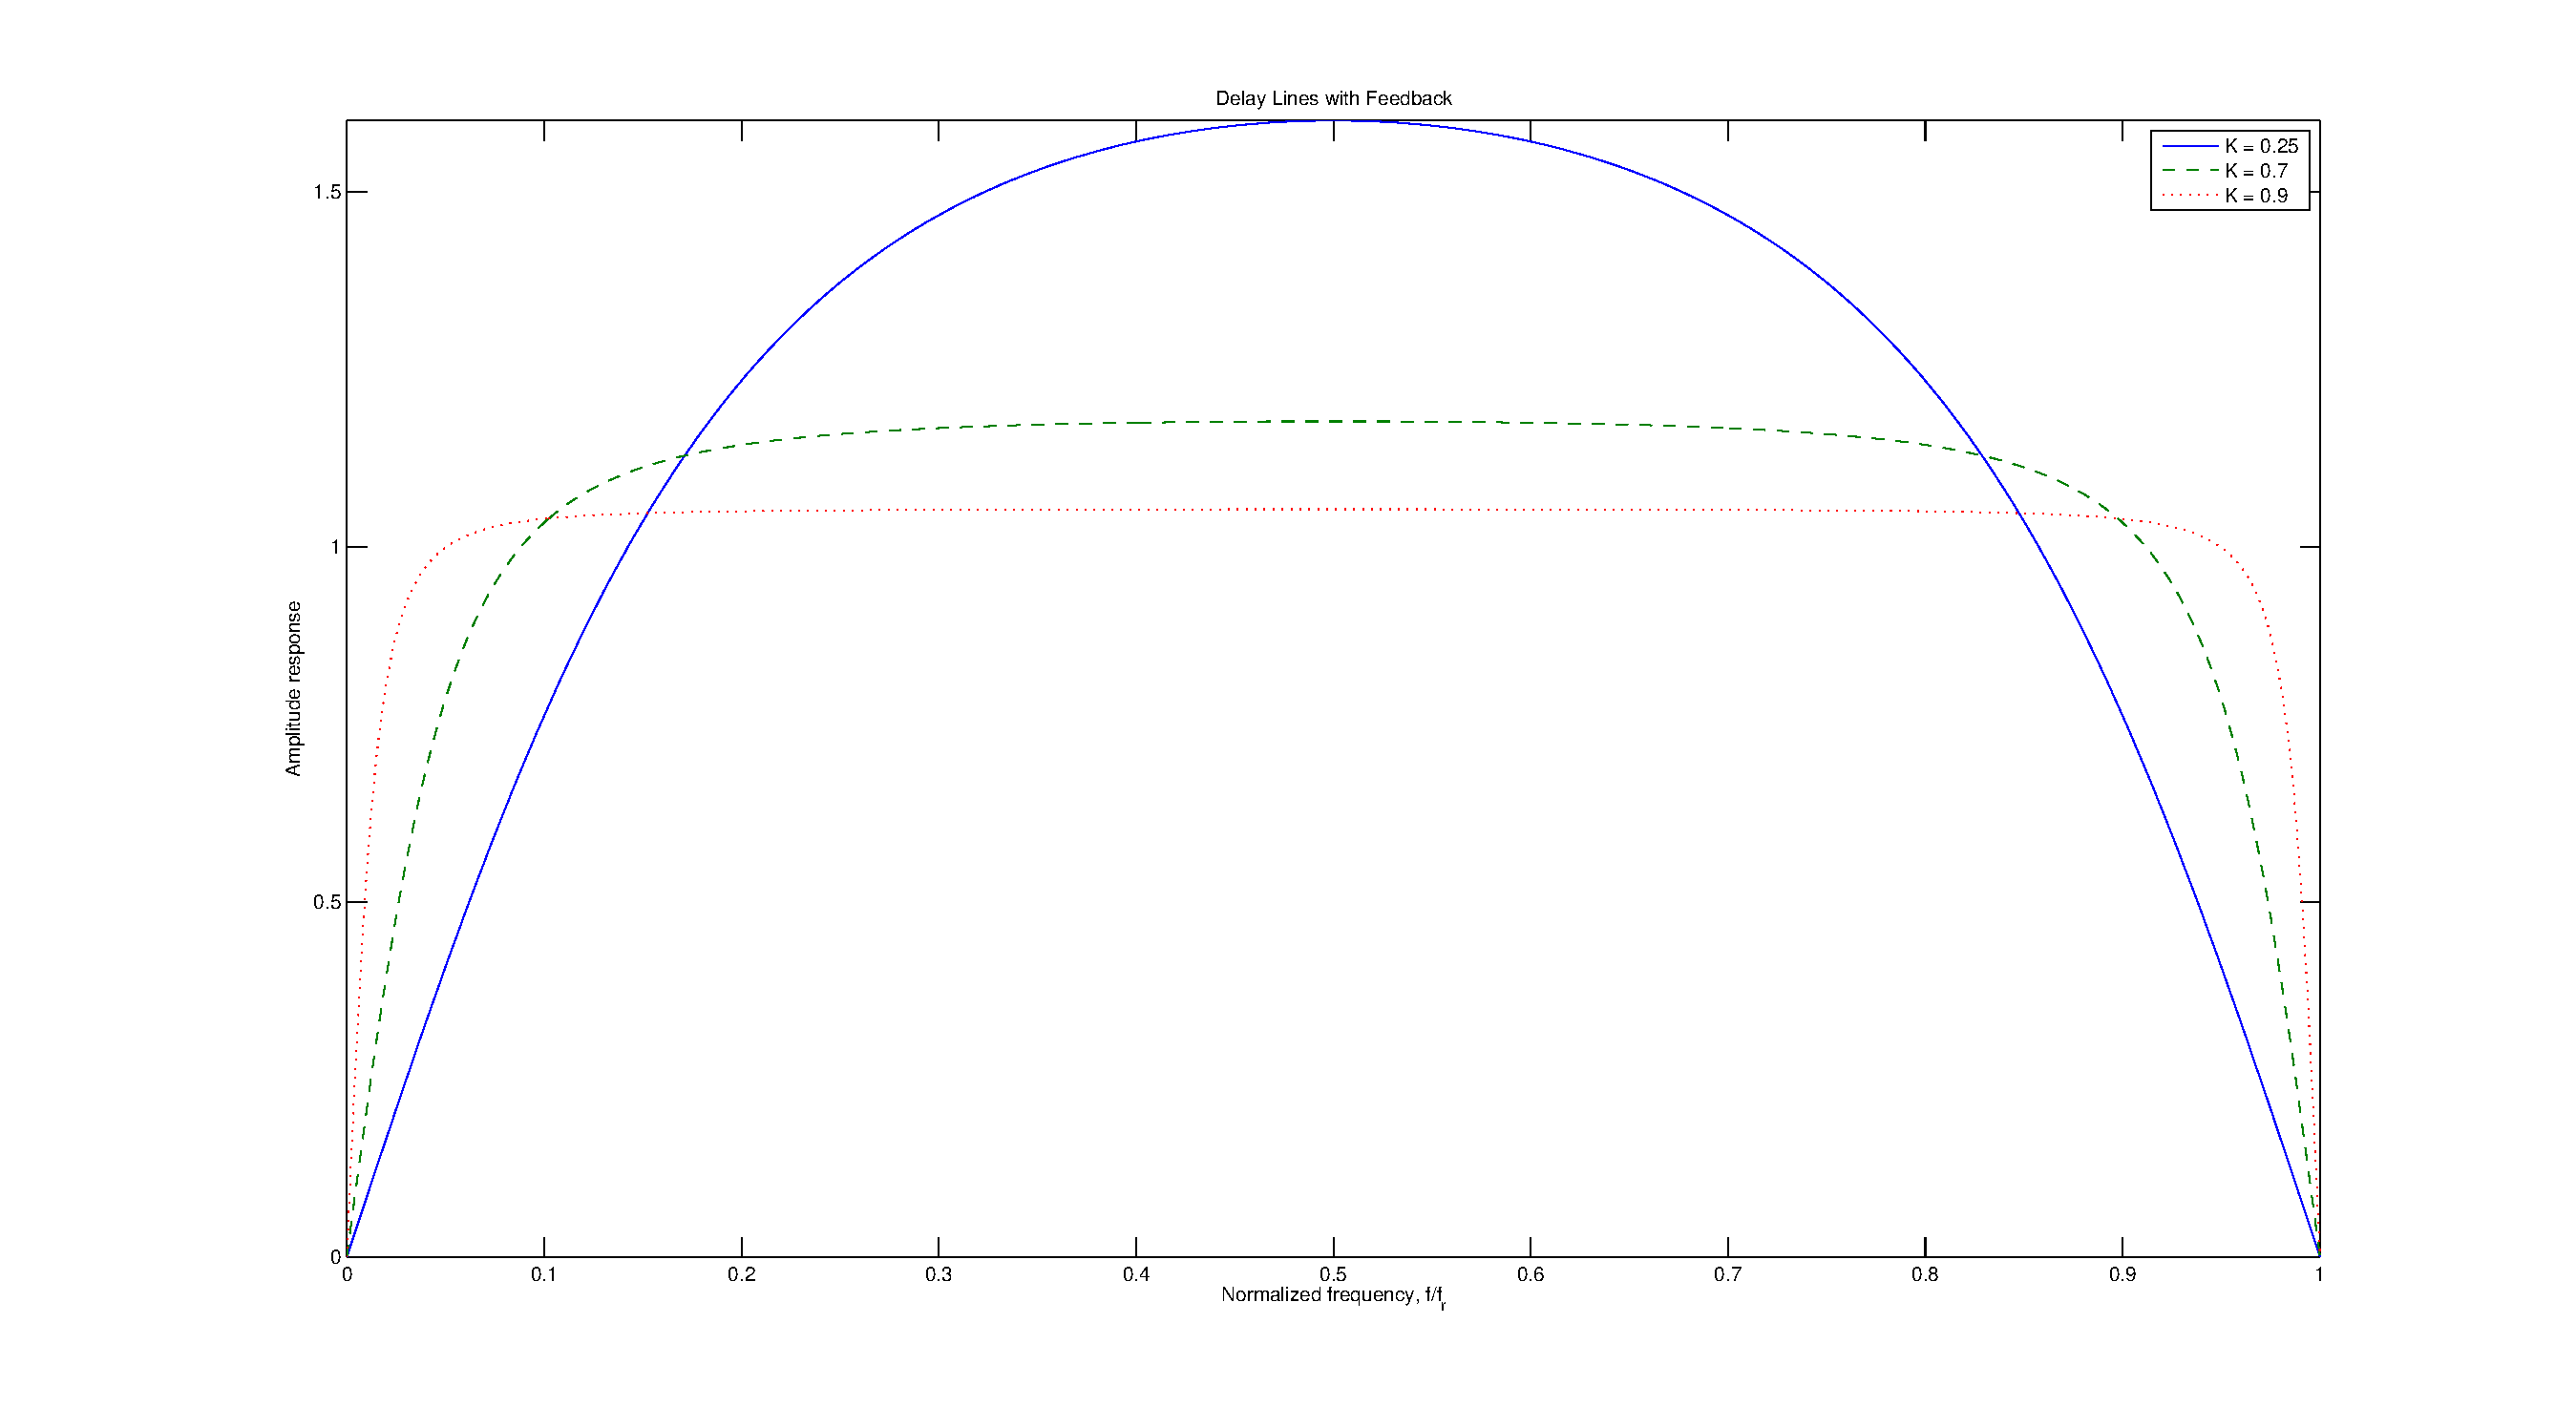
\includegraphics[width=\linewidth]{dlFeedback} \\
	\vfill
	\tiny{Source: Bassem R.~Mahafza. \emph{Radar Systems Analysis and Design Using MATLAB\textsuperscript{\textregistered}}. Chapman \& Hall/CRC, 2000.}
      \end{minipage}
    \end{frame}
   
    
    \begin{frame}{PRF Staggering 4/5}
      \begin{minipage}[t][0.8\textheight][t]{\textwidth}
	\centering
	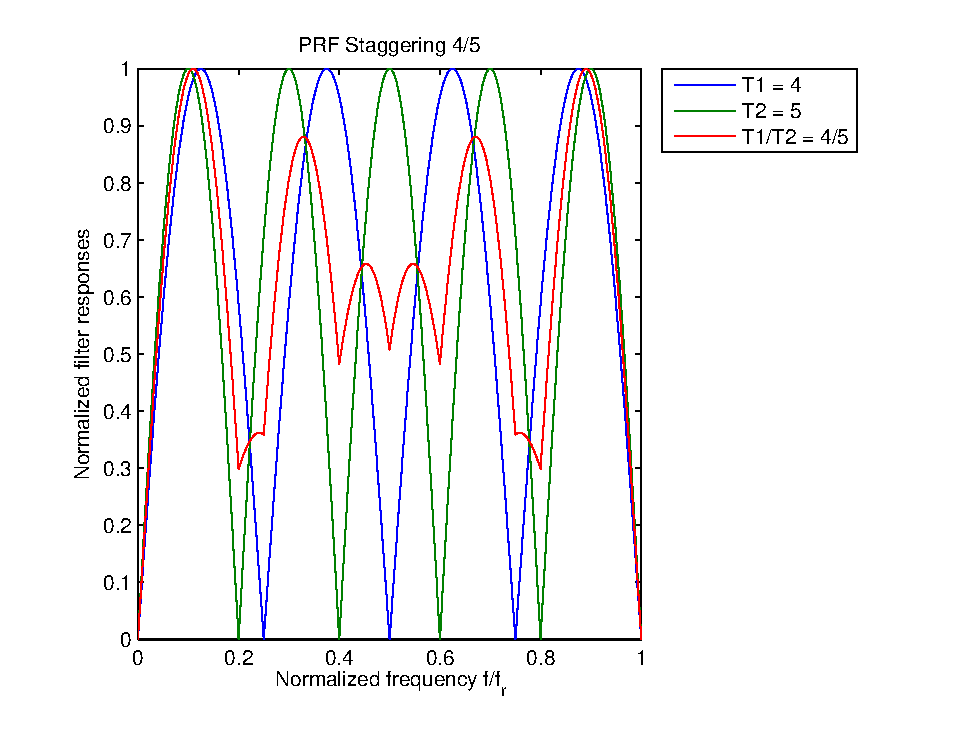
\includegraphics[width=0.8\linewidth]{prfStaggering4_5} \\
	\vfill
	\tiny{Source: Bassem R.~Mahafza. \emph{Radar Systems Analysis and Design Using MATLAB\textsuperscript{\textregistered}}. Chapman \& Hall/CRC, 2000.}
      \end{minipage}
    \end{frame}
    
    
    \begin{frame}{PRF Staggering 33/34}
      \begin{minipage}[t][0.8\textheight][t]{\textwidth}
	\centering
	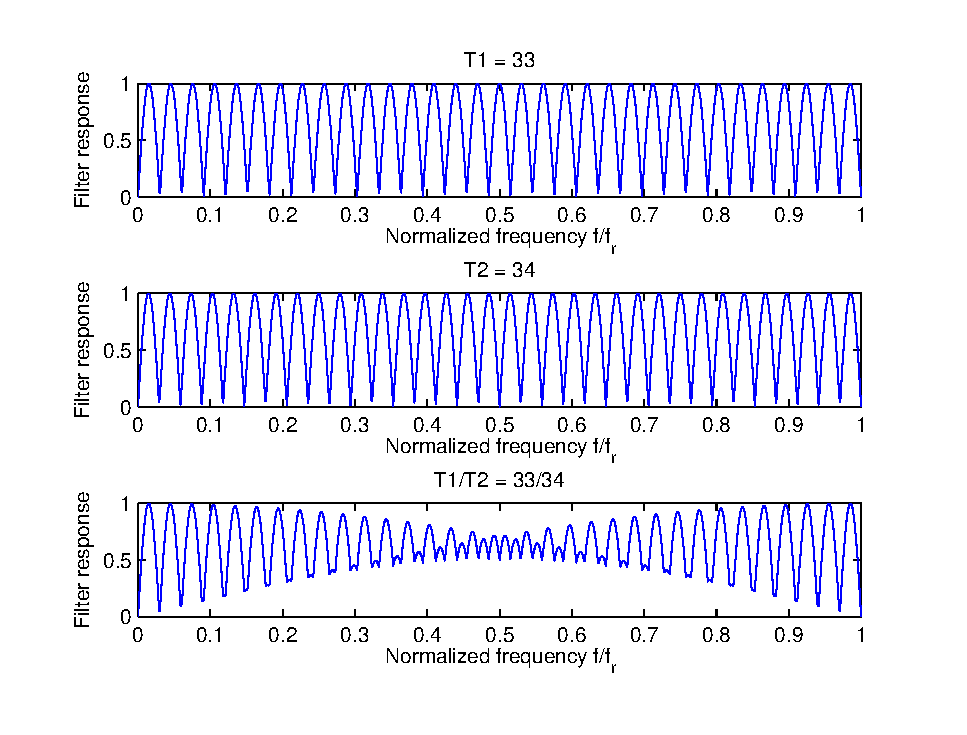
\includegraphics[width=0.7\linewidth]{prfStaggering33_34} \\
	\vfill
	\tiny{Note: The dips in the upper two plots all touch y=0 axis in reality. But since this is a digital plot with just 1000 samples from t=0 to t=1, some of them did not get sampled.} \\
	\tiny{Source: Bassem R.~Mahafza. \emph{Radar Systems Analysis and Design Using MATLAB\textsuperscript{\textregistered}}. Chapman \& Hall/CRC, 2000.}
      \end{minipage}
    \end{frame}
    
   
    \begin{frame}{PRF Staggering 63/64}
      \begin{minipage}[t][0.8\textheight][t]{\textwidth}
	\centering
	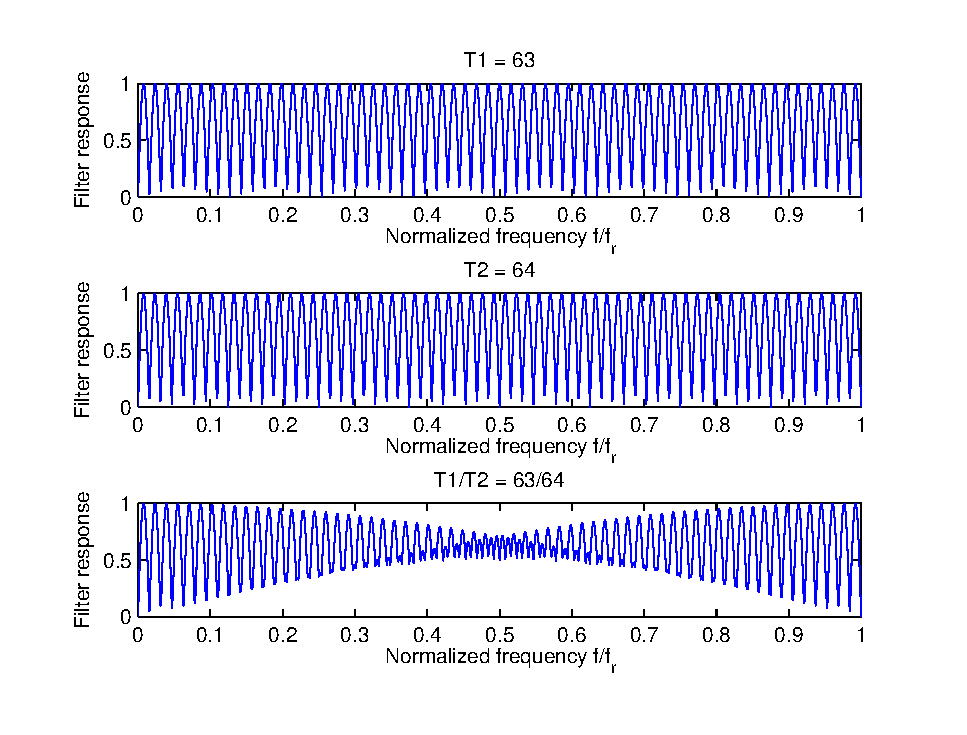
\includegraphics[width=0.7\linewidth]{prfStaggering63_64} \\
	\vfill
	\tiny{Note: The dips in the upper two plots all touch y=0 axis in reality. But since this is a digital plot with just 1000 samples from t=0 to t=1, some of them did not get sampled.} \\
	\tiny{Source: Bassem R.~Mahafza. \emph{Radar Systems Analysis and Design Using MATLAB\textsuperscript{\textregistered}}. Chapman \& Hall/CRC, 2000.}
      \end{minipage}
    \end{frame}
    
    \begin{frame}{First staggered blind speed}
      \begin{minipage}[t][0.8\textheight][t]{\textwidth}
	\begin{align}
	  \frac{n_1}{T_1} & = \frac{n_2}{T_2} = ... = \frac{n_N}{T_N} \nonumber \\
	  v_{blind} & = \frac{n_1 + n_2 + ... + n_N}{N} v_{blind1} \nonumber
	\end{align}
	\vfill
	\tiny{Source: Bassem R.~Mahafza. \emph{Radar Systems Analysis and Design Using MATLAB\textsuperscript{\textregistered}}. Chapman \& Hall/CRC, 2000.}
      \end{minipage}
    \end{frame}

    
    
    \begin{frame}{60Hz input}
      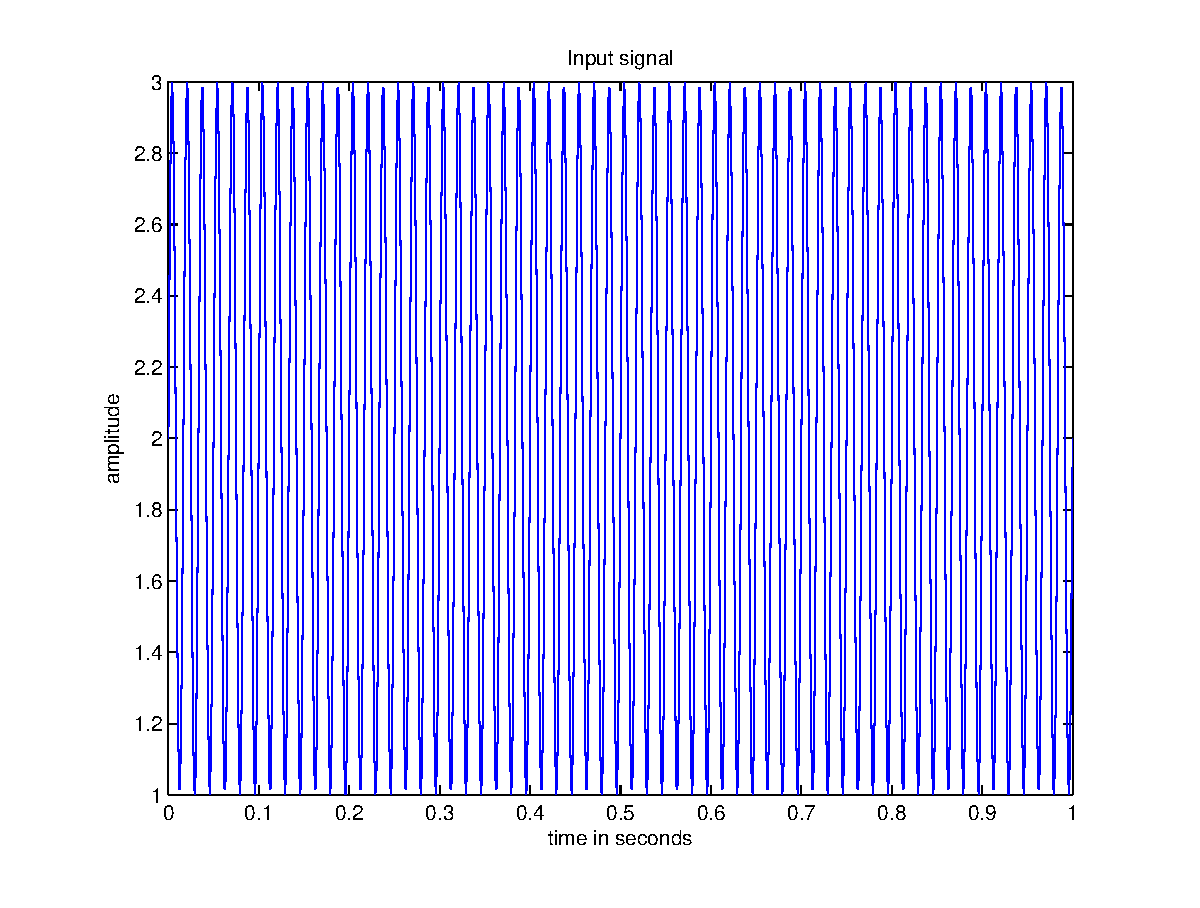
\includegraphics[width=\linewidth]{inputSig60Hz}
    \end{frame}
    
    
    \begin{frame}{Filtered spectrum of 60Hz input}
      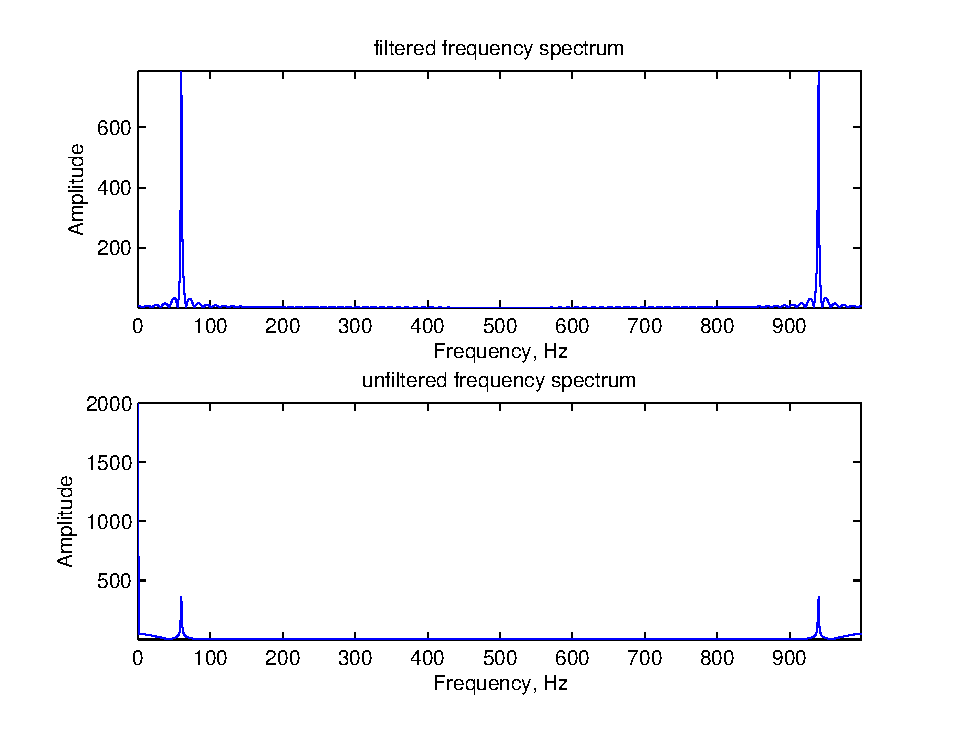
\includegraphics[width=\linewidth]{freqSpec60Hz}
    \end{frame}

    
    \begin{frame}{100Hz input}
      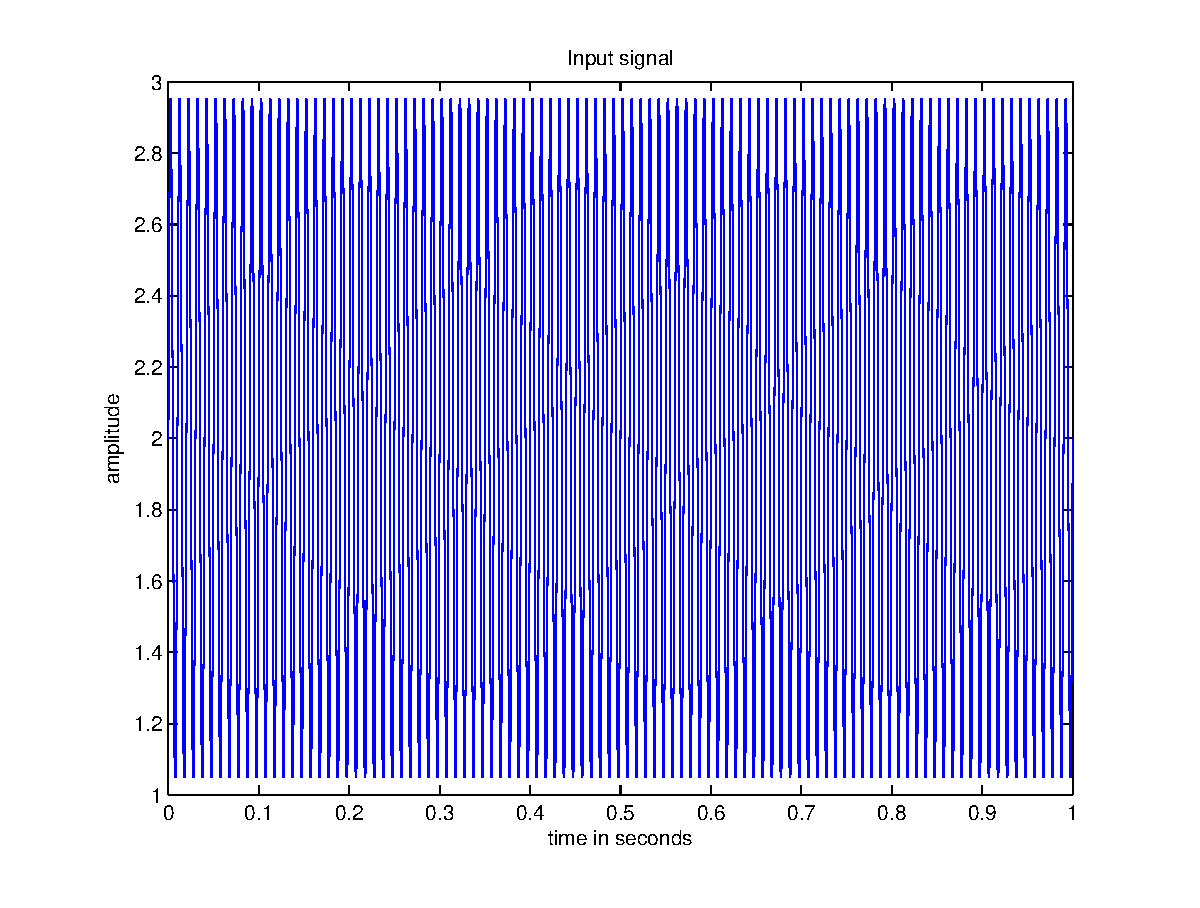
\includegraphics[width=\linewidth]{inputSig100Hz}
    \end{frame}

    
    \begin{frame}{Filtered spectrum of 100Hz input}
      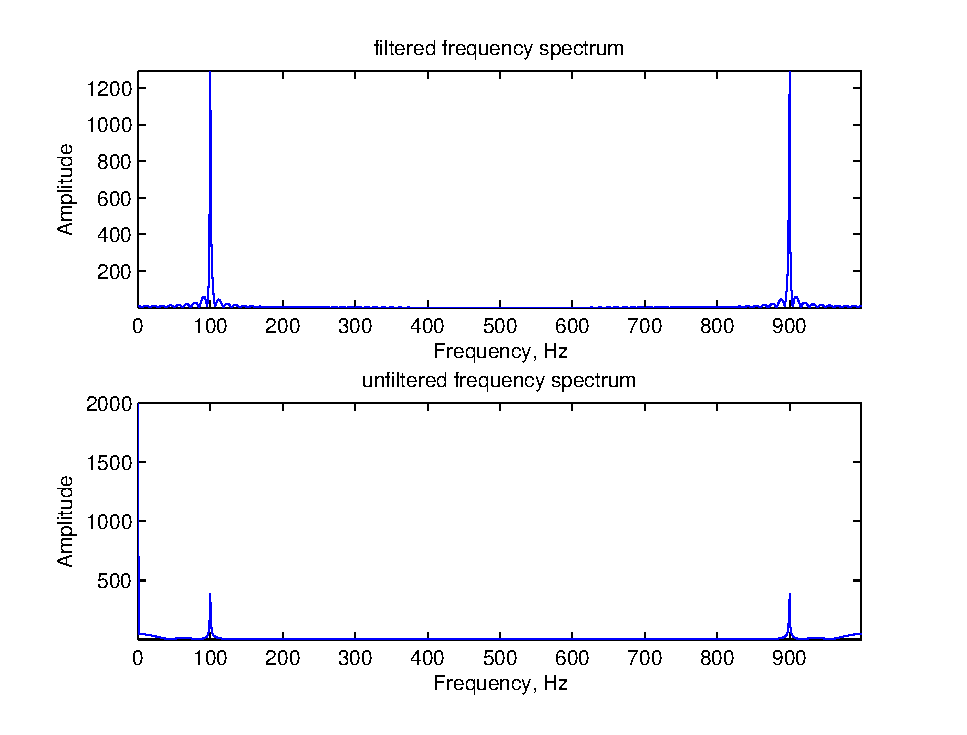
\includegraphics[width=\linewidth]{freqSpec100Hz}
    \end{frame}
    
    
    \begin{frame}{1008Hz input}
      \begin{minipage}[t][0.8\textheight][t]{\textwidth}
	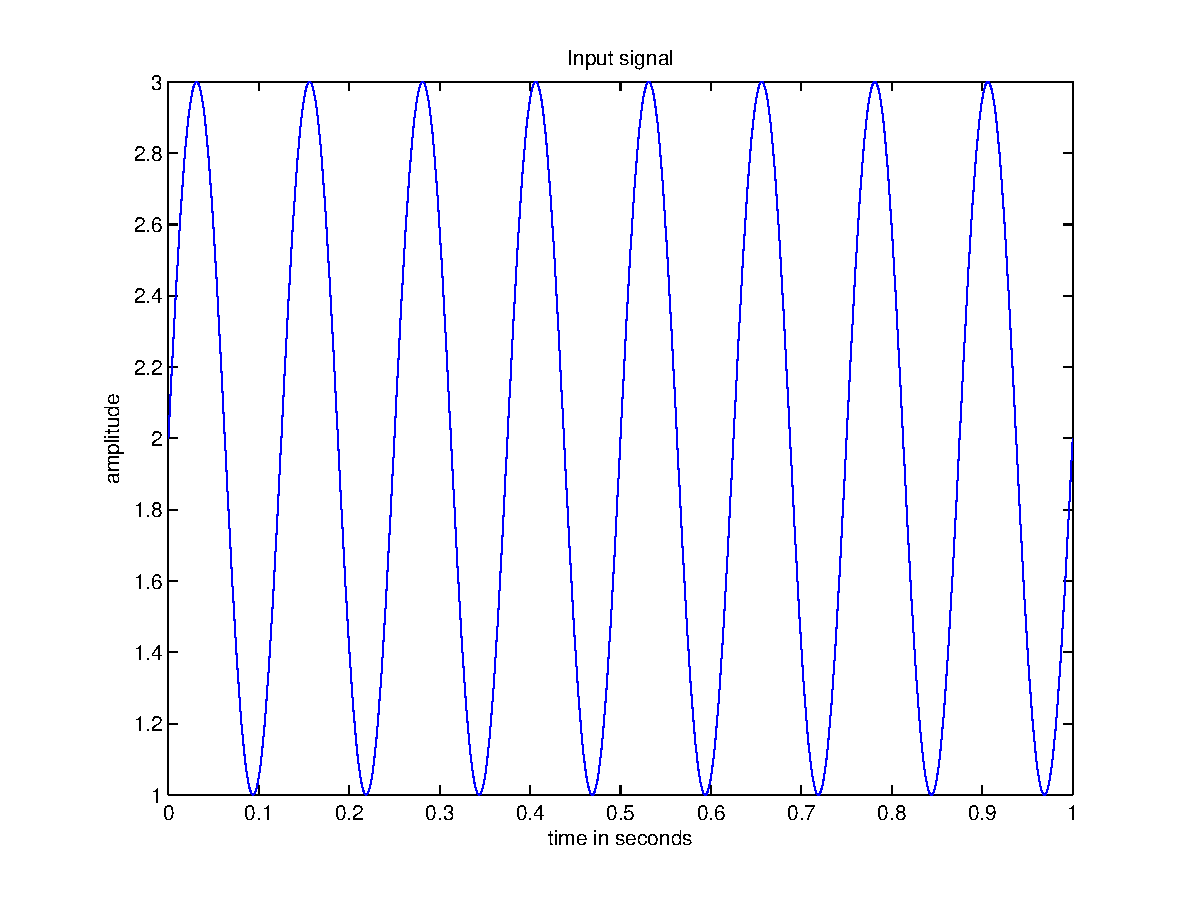
\includegraphics[width=\linewidth]{inputSig1008Hz} \\
	\vfill
	\tiny{Aliased because sampling rate, 1000Hz, is below twice the sampled frequency i.e. 2 * 1008Hz.}
      \end{minipage}
    \end{frame}

    
    \begin{frame}{Filtered spectrum of 1008Hz input}
      \begin{minipage}[t][0.8\textheight][t]{\textwidth}
      \centering
      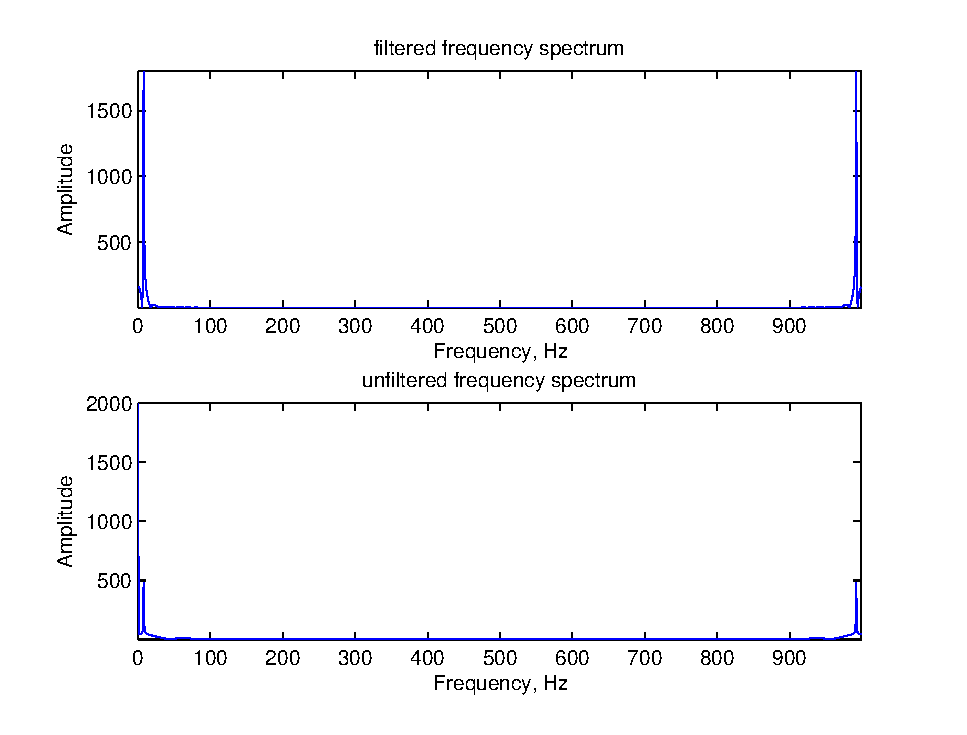
\includegraphics[width=0.7\linewidth]{freqSpec1008Hz} \\
	\vfill
	\tiny{Here we are getting a non-zero filtered output because of aliasing happening due to limited sample rates possible. Ideally we should get a zero output at the frequency in which the blind speed occurs (1008Hz).}
      \end{minipage}
    \end{frame}
    
    
    \begin{frame}{Conclusions}
      \begin{itemize}
       \item Staggering PRFs is the best way to increase the blind speed.
       \item Using higher PRFs increases the blind speed, but it reduces the range of the radar too.
       \item Using staggering ratios like 63/64 gives us an actual first blind speed that is (63+64)/2 or 63.5 times the lowest blind speed among the staggered PRFs.
       \item Similarly by making the staggering ratio closer to 1 and/or by using more than two staggered PRFs, we can get even higher blind speeds without reducing the range of the radar.
      \end{itemize}

    \end{frame}


    \begin{frame}{Digital MTI (I and Q channels)}
      \begin{minipage}[t][0.8\textheight][t]{\textwidth}
 	\begin{figure}[h]
		\centering
		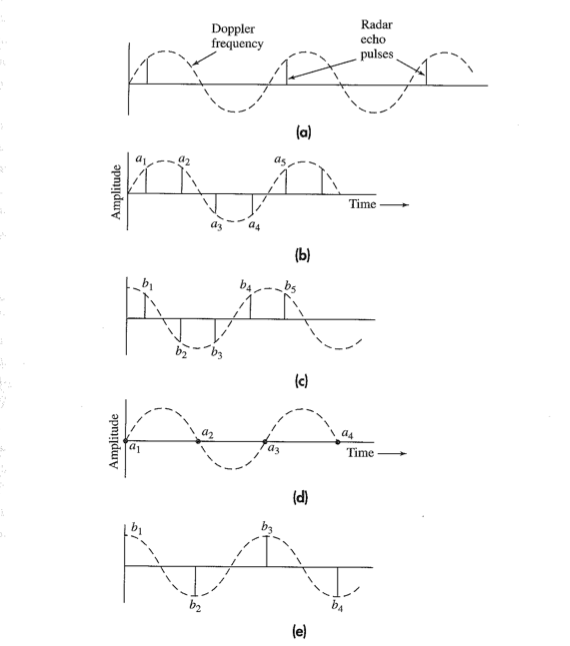
\includegraphics[height=0.7\textheight]{inq}
	\end{figure}
	\vfill
	\tiny{Source: Merrill I.~Skolnik. \emph{Introduction to Radar Systems}. McGraw-Hill, 2001.}
      \end{minipage}
    \end{frame}
    
    \begin{frame}{Digital MTI Processor}
      \begin{minipage}[t][0.8\textheight][t]{\textwidth}
	\begin{figure}[h]
		\centering
		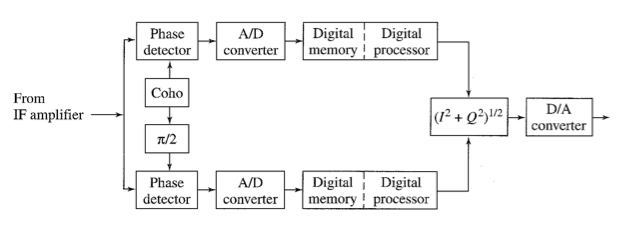
\includegraphics[width=0.9\linewidth]{digitalMTIProcessor}
	\end{figure}
	\vfill
	\tiny{Source: Merrill I.~Skolnik. \emph{Introduction to Radar Systems}. McGraw-Hill, 2001.}
      \end{minipage}
    \end{frame}
    
    \begin{frame}{References}
        
        \begin{itemize}
                 \item Merrill I.~Skolnik. \emph{Introduction to Radar Systems}. McGraw-Hill, 2001.
                 \item Bassem R.~Mahafza. \emph{Radar Systems Analysis and Design Using MATLAB\textsuperscript{\textregistered}}. Chapman \& Hall/CRC, 2000.
                 \item http://en.wikipedia.org/wiki/Moving\_target\_indication
                 \item http://www.radartutorial.eu/11.coherent/co13.en.html
        \end{itemize}
    \end{frame}
    
    
    \begin{frame}[c]
     \begin{center}
       \Huge Thank You
     \end{center}
    \end{frame}

    
\end{document}